\documentclass[]{article}
\usepackage[utf8]{inputenc}
\usepackage[english]{babel}
\usepackage{csquotes}
\usepackage{graphicx}
\usepackage{minted}
\usepackage{amsmath}
\usepackage{amssymb}
\usepackage{parskip}
\usepackage[
backend=biber,
style=alphabetic,
sorting=ynt
]{biblatex}
\addbibresource{references.bib} 
\graphicspath{ {images/} }

%opening
\title{Foundations of Math for ML, part 1}
\author{Hoang Nhat Minh Tran \thanks{Green Global Information Technology JSC}}
\date{\today}

\begin{document}

\maketitle

% The introduction
\begin{abstract}
Machine learning is a set of powerful mathematical tools that enable us, to represent, interpret, and control the complex world around us.
However, even just the word mathematics makes some people feel uneasy and unwelcome to explore the topic.
The purpose of this session is to take you on a tour through the basic maths underlying these methods, focusing in particular on building your intuition rather than worrying too much about the details.
Thanks to the amazing machine learning community, it's actually possible to apply many powerful machine learning methods without understanding very much about the underpinning mathematics, by using open source libraries.
This is great, but problems can arise and without some sense of the language and meaning of the relevant maths, you can struggle to work out what's gone wrong or how to fix it.
The ideal outcome of this session is that it will give you the confidence and motivation to immediately dive into one of the hundreds of boolean applied machine learning courses already available online, and not be intimidated by the matrix notation or the calculus.

In this first module we look at how linear algebra is relevant to machine learning and data science. Then we'll wind up the module with an initial introduction to vectors. Throughout, we're focusing on developing your mathematical intuition, not of crunching through algebra or doing long pen-and-paper examples. For many of these operations, there are callable functions in Python that can do the adding up - the point is to appreciate what they do and how they work so that, when things go wrong or there are special cases, you can understand why and what to do.

\end{abstract}

\section{Learning Objectives}

\begin{itemize}
	\item Recall how machine learning and vectors and matrices are related
	\item Interpret how changes in the model parameters affect the quality of the fit to the training data
	\item Recognize that variations in the model parameters are vectors on the response surface - that vectors are a generic concept not limited to a physical real space
	\item Use substitution / elimination to solve a fairly easy linear algebra problem
	\item Understand how to add vectors and multiply by a scalar number
\end{itemize}

\section{The relationship between machine learning, linear algebra, and vectors and matrices}

\subsection{Motivations for linear algebra}

We're going to look a bit more at the types of problems we might want to solve, and expose what Linear Algebra is and how it might help us to solve them.
The first problem I might think of is one of price discovery.

\begin{equation} \label{eq1}
\begin{split}
2a + 3b & = 8 \\
10a + 1b & = 13
\end{split}
\end{equation}

Say I go shopping on two occasions, and I buy apples and bananas, and the first time I buy two apples and three bananas and they cost eight Euros.
And the second time I buy say, ten apples and one banana, and the cost is 13 Euros.
And the \textbf{As} and the \textbf{Bs} here,
are the price of a \textbf{single apple} and a \textbf{single banana}.
And what I'm going to have to do is \textbf{solve} these what we call \textbf{\textit{simultaneous equations}} in order to discover the price of individual apples and bananas.

Now in the general case of lots of different types of items and lots of shopping trips, then finding out the prices might be quite hard. It might be quite \textit{difficult} to \textit{solve} all these equations \textit{by hand}. So, we might want a computer algorithm to do it for us, in the general case. Now, this is an example of a Linear Algebra problem.

\begin{equation} \label{eq2}
	\begin{bmatrix}
	2 & 3 \\
	10 & 1
	\end{bmatrix}
	\cdot
	\begin{bmatrix}
	a \\
	b
	\end{bmatrix}
	=
	\begin{bmatrix}
	8 \\
	13
	\end{bmatrix}
\end{equation}

I have some \textbf{constant} \textit{linear coefficients} here, these numbers \textit{2, 10, 3, 1}, that relate the \textbf{input} variables A and B, to the \textbf{output} 8 and 13, that is if I think about a vector [a,b], that describes the prices of apples and bananas.

Looking at these different types of mathematical objects, and understanding what they are and how to work with them, these \textit{vectors} and \textit{matrices}. In fact, with neural networks and machine learning, we want the computer in effect \textbf{\textit{not only}} to fit the equation, \textbf{\textit{but also}} to figure out what equation to use. That's a highly inexact description really of what's going on, but it gives the right sort of flavor.

\subsection{Exploring parameter space}

In this exercise, we shall see how it is often convenient to use vectors in machine learning. These could be in the form of data itself, or model parameters, and so on.

\subsubsection{Quiz 1}.

The problem we shall focus on in this exercise is the distribution of heights in a population. If we do a survey of the heights of people in a population, we may get a distribution like this:

\begin{figure}[h]
	\centering
	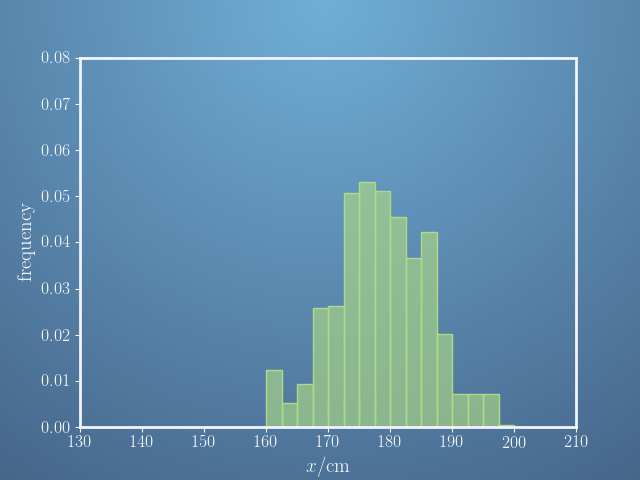
\includegraphics[width=0.5\textwidth]{height_dist}
	\caption{The distribution of heights}
	\label{fig:height_dist}
\end{figure}

This \textit{histogram} \ref{fig:height_dist} indicates how likely it is for anyone in the survey to be in a particular height range. (6 ft is around 183 cm).

This histogram can also be represented by a vector, i.e. a list of numbers. In this case, we record the frequency of people with heights in little groups at 2.5 cm intervals, i.e. between 150 cm and 152.5 cm, between 152.5 cm and 155 cm, and so on. We can define this as the vector $ f $ with components,
\begin{equation} \label{f_vector}
	f =
	\begin{bmatrix}
		f_{150.0, 152.5} \\
		f_{152.5, 155.0} \\
		f_{155.0, 157.5} \\
		f_{157.5, 160.0} \\
		\vdots
	\end{bmatrix}
\end{equation}

These vector components are the sizes of each bar in the histogram. Of the following statements, select all that you think are true.

\begin{itemize}
	\item[$\square$] If another sample was taken under the same conditions, the frequencies would be exactly the same.
	\item[$\square$] If another sample was taken under the same conditions, the frequencies should be broadly similar.
	\item[$\square$] There are at least 10 elements in the frequency vector, f.
	\item[$\square$] None of the other statements.
	\item[$\square$] No one in the world is less than 160 cm tall. 
\end{itemize}

\subsubsection{Quiz 2}

One of the tasks of machine learning is to fit a model to data in order to represent the underlying distribution.

For the heights of a population, a model we may use to predict frequencies is the Normal (or Gaussian) distribution. This is a model for a bell-shaped curve, which looks like this,

\begin{figure}[h]
	\centering
	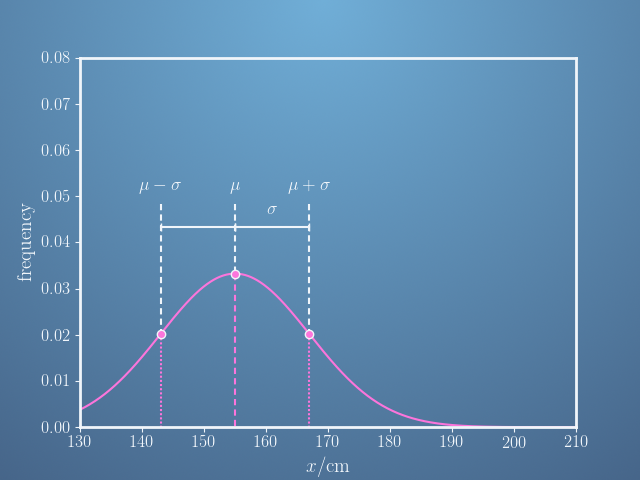
\includegraphics[width=0.5\textwidth]{underlying_dist}
	\caption{The underlying distribution}
	\label{fig:underlying_dist}
\end{figure}

It has the slightly complicated equation,

\begin{equation}
	g(x) = \frac{1}{\sigma\sqrt{2\pi}}\exp\left(-\frac{(x-
		\mu)^2}{2\sigma^2}\right)
\end{equation}
the exact form of which is unimportant, except that it is dependent on two parameters, the $ mean $, $ \mu $, where the curve is centered, and the \textit{standard deviation}, $ \sigma $, which is the characteristic width of the bell curve (measured from the mean).

We can put these two parameters in a vector, $ p = \begin{bmatrix}
\mu \\
\sigma
\end{bmatrix} $

Pick the parameter vector $ p $ which best describes the distribution pictured.

\begin{itemize}
	\item[$\square$] $ p = \begin{bmatrix}
		167 \\
		24
		\end{bmatrix} $
	\item[$\square$] $ p = \begin{bmatrix}
		155 \\
		12
		\end{bmatrix} $
	\item[$\square$] $ p = \begin{bmatrix}
		143 \\
		167
		\end{bmatrix} $
	\item[$\square$] $ p = \begin{bmatrix}
		155 \\
		3
		\end{bmatrix} $
	\item[$\square$] $ p = \begin{bmatrix}
		167 \\
		2
		\end{bmatrix} $
\end{itemize}

\subsubsection{Quiz 3}.

Pick the Normal distribution that corresponds the closest to the parameter vector $ p= \begin{bmatrix}
3 \\
3
\end{bmatrix} $

\begin{itemize}
	\item[$\square$] 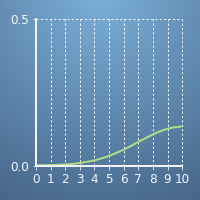
\includegraphics[width=0.5\textwidth]{quiz3_a}
	\item[$\square$] 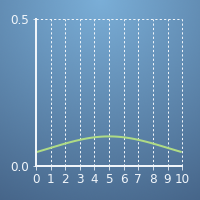
\includegraphics[width=0.5\textwidth]{quiz3_b}
	\item[$\square$] 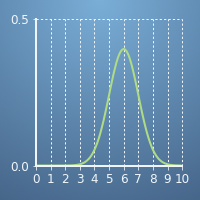
\includegraphics[width=0.5\textwidth]{quiz3_c}
	\item[$\square$] 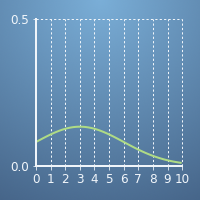
\includegraphics[width=0.5\textwidth]{quiz3_d}
\end{itemize}

\textbf{Quiz 4}. A model allows us to predict the data in a distribution. In our example we can start with a parameter vector $ p $ and convert it to a vector of expected frequencies $ g_p $, for example, $ g_p =
\begin{bmatrix}
	f_{150.0, 152.5} \\
	f_{152.5, 155.0} \\
	f_{155.0, 157.5} \\
	f_{157.5, 160.0} \\
	\vdots
\end{bmatrix} $

A model is only considered good if it fits the measured data well. Some specific values for the parameters will be better than others for a model. We need a way fit a model's parameters to data and quantify how good that fit is.

One way of doing so is to calculate the "residuals", which is the difference between the measured data and the modeled prediction for each histogram bin.

This is illustrated below. The model is shown in pink, the measured data is shown in orange and where they overlap is shown in green. The height of the pink and orange bars are the residuals.

\begin{figure}[h]
	\centering
	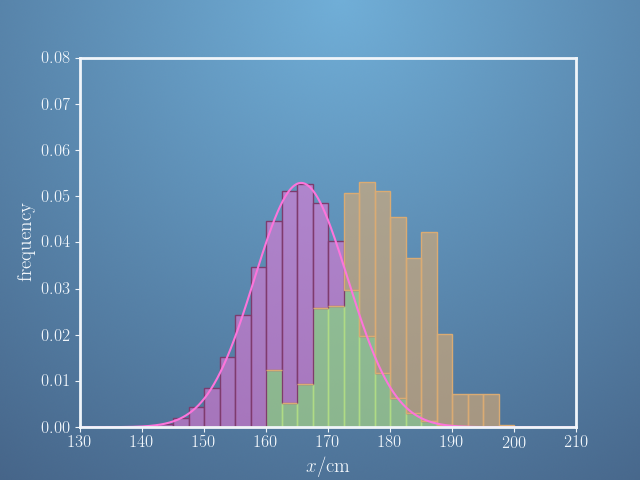
\includegraphics[width=\textwidth]{residuals}
	\caption{The model and the measured data}
	\label{fig:residuals}
\end{figure}

A better fit would have as much overlap as it can, reducing the residuals as much as possible. How could the model be improved to give the best fit to the data?

\begin{itemize}
	\item[$\square$] Increase the standard deviation, $ \sigma $.
	\item[$\square$] Keep the standard deviation, $ \sigma $, approximately the same.
	\item[$\square$] Decrease the mean, $ \mu $.
	\item[$\square$] Increase the mean, $ \mu $.
	\item[$\square$] Decrease the standard deviation, $ \sigma $.
	\item[$\square$] Keep the mean, $ \mu $, approximately the same.
\end{itemize}

\subsubsection{Quiz 5}.

The performance of a model can be quantified in a single number. One measure we can use is the \textit{Sum of Squared Residuals}, SSR. Here we take all of the residuals (the difference between the measured and predicted data), square them and add them together.

In the language of vectors we can write this as, $ SSR(p)=|f-g_p|^2 $ , which will be explained further on in this course.

Since each parameter vector $ p $ represents a different bell curve, each with its own value for the sum of squared residuals, $ SSR $, we can draw the surface of $ SSR $ values over the space spanned by p, such as $ \mu $ and $ \sigma $ in this example.

Here is an illustration of this surface for our data.

\begin{figure}[h]
	\centering
	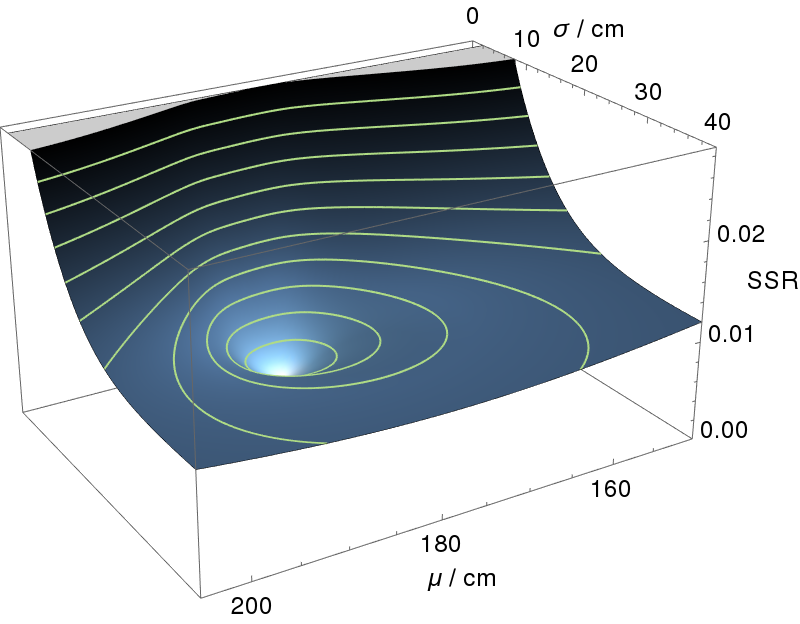
\includegraphics[width=0.5\textwidth]{quiz5_a}
	\caption{The surface of data}
	\label{fig:quiz5_a}
\end{figure}

Every point on this surface represents the $ SSR $ of a choice of parameters, with some bell curves performing better at representing the data than others.

We can take a ‘top-down’ view of the surface, and view it as a contour map, where each of the contours (in green here) represent a constant value for the $ SSR $.

\begin{figure}[h]
	\centering
	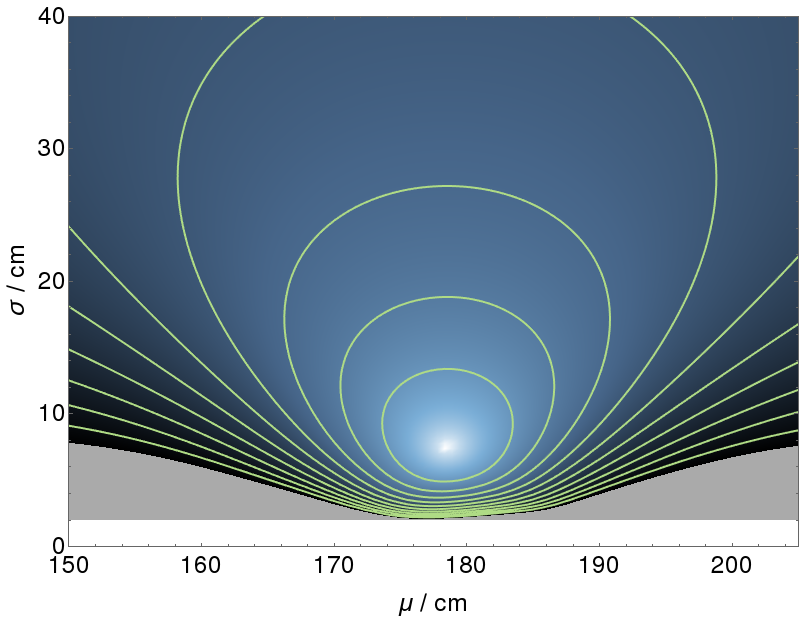
\includegraphics[width=0.5\textwidth]{quiz5_b}
	\caption{The surface of data in top-down}
	\label{fig:quiz5_b}
\end{figure}

The goal in machine learning is to find the parameter set where the model fits the data as well as it possibly can. This translates into finding the lowest point, the global minimum, in this space.

Select all true statements below.

\begin{itemize}
	\item[$\square$] At the minimum of the surface, the model exactly matches the measured data.
	\item[$\square$] None of the other statements.
	\item[$\square$] You get the same model by following along a contour line.
	\item[$\square$] Moving at right angles to contour lines in the parameter space will have the greatest effect on the fit than moving in other directions.
	\item[$\square$] Each point on the surface represents a set of parameters $ p = \begin{bmatrix}
		\mu \\
		\sigma
	\end{bmatrix}$.
\end{itemize}

\subsection{Solving some simultaneous equations}

\subsubsection{Quiz 1}.

In this quiz you'll be reminded of how to solve linear simultaneous equations as a way to practice some basic linear algebra. Some of the ideas presented here will be relevant later in the course.

Solving simultaneous equations is the process of finding the values of the variables (here $ x $ and $ y $) that satisfy the system of equations. Let's start with the simplest type of simultaneous equation, where we already know all but one of the variables:

\begin{equation} \label{}
\begin{split}
	3x - y = 2 \\
	x = 4
\end{split}
\end{equation}

Substitute the value of xxx into the first equation to find yyy, then select the correct values of $ x $ and $ y $ below.

\begin{itemize}
	\item[$\square$] $ x = 4, y = 14 $
	\item[$\square$] $ x = 4, y = 2 $
	\item[$\square$] $ x = 4, y = -10 $
	\item[$\square$] $ x = 4, y = 10 $
\end{itemize}

\subsubsection{Quiz 2}.

The first goal when solving simple simultaneous equations should be to isolate one of the variables. For example, try taking the second equation away from the first to solve the following pair of equations:

\begin{equation} \label{}
\begin{split}
3x - 2y = 7 \\
2x - 2y = 2
\end{split}
\end{equation}

What value did you find for $ x $? Now substitute $ x $ into one of the equations to find $ y $, and select the correct pair below:

\begin{itemize}
	\item[$\square$] $ x = 1, y = -4 $
	\item[$\square$] $ x = 3, y = 1 $
	\item[$\square$] $ x = 7, y = 7 $
	\item[$\square$] $ x = 5, y = 4 $
\end{itemize}

\subsubsection{Quiz 3}.

This method is called \textit{elimination}, and you can use it even when the coefficients, the numbers in front of $ x $ and $ y $, aren't the same.

\begin{equation} \label{}
\begin{split}
3x - 2y = 4 \\
6x + 3y = 15
\end{split}
\end{equation}

Select the correct values of $ x $ and $ y $ below:

\begin{itemize}
	\item[$\square$] $ x = 4, y = -2 $
	\item[$\square$] $ x = 3, y = 1 $
	\item[$\square$] $ x = 2, y = 1 $
	\item[$\square$] $ x = 1, y = 2 $
\end{itemize}

% \subsection{Operations with vectors}

\section{Data Manipulation}

It is impossible to get anything done if we cannot manipulate data. Generally, there are two important things we need to do with data: (i) acquire it and (ii) process it once it is inside the computer.  There is no point in acquiring data if we do not even know how to store it, so let’s get our hands dirty first by playing with synthetic data. We will start by introducing the Tensor, PyTorch’s primary tool for storing and transforming data.  If you have worked with NumPy before, you will notice that Tensor are, by design, similar to NumPy’s multi-dimensional array.  However, they confer a few key advantages.  First, Tensor supports asynchronous computation on CPU, GPU, and distributed cloud architectures. Second,they provide support for automatic differentiation. These properties make Tensor indispensable for deep learning.

\subsection{Getting Started}

Throughout this section, we are aiming to get you up and running with the basic functionality. Do not worry if you do not understand all of the basic math, like element-wise operations or normal distributions. We begin by importing PyTorch.

\begin{minted}[frame=single]{python}
import torch
\end{minted}

Tensors represent (possibly multi-dimensional) arrays of numerical values. Tensors with one axis correspond (in math-speak) to \textit{vectors}. Tensors with two axes correspond to \textit{matrices}. For arrays with more than two axes, mathematicians do not have special names—they simply call them \textit{tensors}.

The simplest object we can create is a vector. To start, we can use \textbf{arange} to create a row vector with 12 consecutive integers.

\begin{minted}[frame=single]{python}
x = torch.arange(12)
x
\end{minted}

\begin{minted}[frame=single]{python}
tensor([ 0,  1,  2,  3,  4,  5,  6,  7,  8,  9, 10, 11])
\end{minted}

We can get the Tensor instance shape through the \textbf{size} property.

\begin{minted}[frame=single]{python}
x.size()
\end{minted}

\begin{minted}[frame=single]{python}
torch.Size([12])
\end{minted}

We use the \textbf{view} function to change the shape of one (possibly multi-dimensional) array, to another that contains the same number of elements. For example, we can transform the shape of our line vector \textbf{x} to (3,4), which contains the same values but interprets them as a matrix containing 3 rows and 4 columns. Note that although the shape has changed, the elements in \textbf{x} have not. Moreover, the size remains the same.

\begin{minted}[frame=single]{python}
x.view(3, 4)
x
\end{minted}

\begin{minted}[frame=single]{python}
tensor([[ 0,  1,  2,  3],
	[ 4,  5,  6,  7],
	[ 8,  9, 10, 11]])
\end{minted}

Reshaping by manually specifying each of the dimensions can get annoying.  Once we know one of the dimensions, why should we have to perform the division our selves to determine the other? For example,above, to get a matrix with 3 rows, we had to specify that it should have 4 columns (to account for the12 elements). Fortunately, Tensor can automatically work out one dimension given the other. We can invoke this capability by placing $ -1 $ for the dimension that we would like Tensor to automatically infer. In our case, instead of \textbf{x.view(3, 4)}, we could have equivalently used \textbf{x.view(-1, 4)} or \textbf{x.view(3, -1)}.

To create a Tensor representing a tensor with all elements set to 0 and a shape of (2, 3, 4) we can invoke:

\begin{minted}[frame=single]{python}
torch.zeros(2,3,4)
\end{minted}

\begin{minted}[frame=single]{python}
tensor([[[0., 0., 0., 0.],
	 [0., 0., 0., 0.],
	 [0., 0., 0., 0.]],
	
	 [[0., 0., 0., 0.],
	 [0., 0., 0., 0.],
	 [0., 0., 0., 0.]]])
\end{minted}

We can create tensors with each element set to 1 works via

\begin{minted}[frame=single]{python}
torch.ones(2,3,4)
\end{minted}

\begin{minted}[frame=single]{python}
tensor([[[1., 1., 1., 1.],
	 [1., 1., 1., 1.],
	 [1., 1., 1., 1.]],
	
	 [[1., 1., 1., 1.],
	 [1., 1., 1., 1.],
	 [1., 1., 1., 1.]]])
\end{minted}

We can also specify the value of each element in the desired Tensor by supplying a Python list containing the numerical values.

\begin{minted}[frame=single]{python}
x = torch.tensor([[2, 1, 4, 3],
	          [1, 2, 3, 4],
	          [4, 3, 2, 1]])
x
\end{minted}

\begin{minted}[frame=single]{python}
tensor([[2, 1, 4, 3],
	[1, 2, 3, 4],
	[4, 3, 2, 1]])
\end{minted}

In some cases, we will want to randomly sample the values of each element in the Tensor according to some known probability distribution. This is especially common when we intend to use the array as a parameter in a neural network. The following snippet creates an Tensor with a shape of (3,4). Each of its elements is randomly sampled in a normal distribution with zero mean and unit variance

\begin{minted}[frame=single]{python}
torch.rand(3,4)
\end{minted}

\begin{minted}[frame=single]{python}
tensor([[0.3600, 0.7597, 0.2731, 0.1179],
	[0.7362, 0.0399, 0.5782, 0.5169],
	[0.2102, 0.8529, 0.0264, 0.3641]])
\end{minted}

\subsection{Operations}

Oftentimes, we want to apply functions to arrays. Some of the simplest and most useful functions are the element-wise functions. These operate by performing a single scalar operation on the corresponding elements of two arrays. We can create an element-wise function from any function that maps from the scalars to the scalars. In math notations we would denote such a function as $ f: \mathbb{R} \rightarrow \mathbb{R} $. Given any two vectors \textbf{u} and \textbf{v} of the \textit{same} shape, and the function f, we can produce a vector $ c=F(u;v) $ by setting $ c_i \leftarrow (u_i; v_i) $ for all $ i $. In PyTorch, the common standard arithmetic operators (+,-,/,*,**) have all been \textit{lifted} to element-wise operations for identically-shaped tensors of arbitrary shape. We can call element-wise operations on any two tensors of the same shape, including matrices.

\begin{minted}[frame=single]{python}
x = torch.tensor([1, 2, 4, 8])
y = torch.ones_like(x) * 2	# result has the same size
print(f'x = {x}')
print(f'x + y {x+y}')
print(f'x - y {x-y}')
print(f'x * y {x*y}')
print(f'x / y {x/y}')
\end{minted}

\begin{minted}[frame=single]{python}
x = tensor([1, 2, 4, 8])
x + y tensor([ 3,  4,  6, 10])
x - y tensor([-1,  0,  2,  6])
x * y tensor([ 2,  4,  8, 16])
x / y tensor([0, 1, 2, 4])
\end{minted}

In addition to computations by element, we can also perform matrix operations, like matrix multiplication using the $ matmul $ function. Next, we will perform matrix multiplication of $ x $ and the transpose of $ y $. We define $ x $ as a matrix of 3 rows and 4 columns, and $ y $ is transposed into a matrix of 4 rows and 3 columns. The two matrices are multiplied to obtain a matrix of 3 rows and 3 columns.

\begin{minted}[frame=single]{python}
x = torch.arange(12).view(3,4)
y = torch.tensor([[2,1,4,3], [1,2,3,4], [4,3,2,1]])
torch.matmul(x, y.T) 
\end{minted}

\begin{minted}[frame=single]{python}
tensor([[ 18,  20,  10],
	[ 58,  60,  50],
	[ 98, 100,  90]])
\end{minted}

We can also merge multiple Tensors. For that, we need to tell the system along which dimension to merge. The example below merges two matrices along dimension 0 (along rows) and dimension 1 (along columns)respectively

\begin{minted}[frame=single]{python}
torch.cat((x, y), dim=0)
torch.cat((x, y), dim=1)
\end{minted}

\begin{minted}[frame=single]{python}
tensor([[ 0,  1,  2,  3,  2,  1,  4,  3],
	[ 4,  5,  6,  7,  1,  2,  3,  4],
	[ 8,  9, 10, 11,  4,  3,  2,  1]])
\end{minted}

Sometimes, we may want to construct binary Tensors via logical statements. Take $ x $ == $ y $ as an example. If $ x $ and $ y $ are equal for some entry, the new Tensor has a value of 1 at the same position; otherwise it is 0

\begin{minted}[frame=single]{python}
x == y
\end{minted}

\begin{minted}[frame=single]{python}
tensor([[False,  True, False,  True],
	[False, False, False, False],
	[False, False, False, False]])
\end{minted}

Summing all the elements in the Tensor yields an Tensor with only one element.

\begin{minted}[frame=single]{python}
x.sum()
\end{minted}

\begin{minted}[frame=single]{python}
tensor(66)
\end{minted}

We can transform the result into a scalar in Python using  the asscalar function. In the following example,the $ l_2 $ norm of $ x $ yields a single element Tensor. The final result is transformed into a scalar.

\begin{minted}[frame=single]{python}
x = torch.arange(12, dtype=torch.float32).view(3,4)
x.norm().item()
\end{minted}

\begin{minted}[frame=single]{python}
22.494443893432617
\end{minted}

\subsection{Broadcast Mechanism}

In the above section, we saw how to perform operations on two Tensors of the same shape. When their shapes differ, a broadcasting mechanism may be triggered analogous to NumPy: first, copy the elements appropriately so that the two Tensors have the same shape, and then carry out operations by element.

\begin{minted}[frame=single]{python}
a = torch.arange(3).view(3,1)
b = torch.arange(2).view(1,2)
a, b
\end{minted}

\begin{minted}[frame=single]{python}
(tensor([[0],
	 [1],
	 [2]]), tensor([[0, 1]]))
\end{minted}

Since $ a $ and $ b $ are (3x1) and (1x2) matrices respectively, their shapes do not match up if we want to add them. Tensor addresses this by \textbf{\textit{broadcasting}} the entries of both matrices into a larger (3x2) matrix as follows: for matrix $ a $ it replicates the columns, for matrix $ b $ it replicates the rows before adding up both element-wise.

\begin{minted}[frame=single]{python}
a + b
\end{minted}

\begin{minted}[frame=single]{python}
tensor([[0, 1],
	[1, 2],
	[2, 3]])
\end{minted}

\subsection{Indexing and Slicing}

Just like in any other Python array, elements in an Tensor can be accessed by its index. In good Python tradition the first element has index 0 and ranges are specified to include the first but not the last element.By this logic $ 1:3 $ selects the second and third element. Let’s try this out by selecting the respective rows in a matrix.

\begin{minted}[frame=single]{python}
x[1:3]
\end{minted}

\begin{minted}[frame=single]{python}
tensor([[ 0.,  1.,  2.,  3.],
	[ 4.,  5.,  6.,  7.],
	[ 8.,  9., 10., 11.]])
\end{minted}

Beyond reading, we can also write elements of a matrix.

\begin{minted}[frame=single]{python}
x[1, 2] = 9
x
\end{minted}

\begin{minted}[frame=single]{python}
tensor([[ 0.,  1.,  2.,  3.],
	[ 4.,  5.,  9.,  7.],
	[ 8.,  9., 10., 11.]])
\end{minted}

If we want to assign multiple elements the same value, we simply index all of them and then assign them the value. For instance, $ [0:2, :] $ accesses the first and second rows. While we discussed indexing for matrices,this obviously also works for vectors and for tensors of more than 2 dimensions.

\begin{minted}[frame=single]{python}
x[0:2, :] = 12
x
\end{minted}

\begin{minted}[frame=single]{python}
tensor([[12., 12., 12., 12.],
	[12., 12., 12., 12.],
	[ 8.,  9., 10., 11.]])
\end{minted}

\subsection{Mutual Transformation of Tensor and NumPy}

Converting PyTorch Tensors to and from NumPy is easy. The converted arrays do not \textit{share} memory. This minor inconvenience is actually quite important: when you perform operations on the CPU or one of the GPUs, you do not want PyTorch having to wait whether NumPy might want to be doing something else with the same chunk of memory. The \textit{from\textunderscore numpy} and \textit{numpy} functions do the trick.

\begin{minted}[frame=single]{python}
import torch
import numpy as np

a = x.numpy()
print(type(a))
b = torch.from_numpy(a)
print(type(b))
\end{minted}

\begin{minted}[frame=single]{python}
<class 'numpy.ndarray'>
<class 'torch.Tensor'>
\end{minted}

\subsection{Exercise}

\begin{enumerate}
	\item Run the code in this section. Change the conditional statement $ x == y $ in this section to $ x < y $ or $ x > y $, and then see what kind of Tensor you can get.
	\item Replace the two Tensors that operate by element in the \textit{broadcast mechanism} with other shapes, e.g. three dimensional (3D) tensors. Is the result the same as expected?
	\item Rewrite $ c = torch.matmul(a, b.T) + c $ in the most memory efficient manner.
\end{enumerate}

\section{Recap}

In this first module of our course on Linear Algebra, we first looked at the problem of data, that our world has so much of it. And then if we could figure out how to analyze and use it, we could really solve problems in the world.

Secondly, we've moved on to look at some example problems, the problem of solving some simultaneous equations. For example, to discover the price of things in the apples and bananas problem, or the problem of fitting a model equation with some fitting parameters we want, to optimize against some data.

We've then said that both of these problems are going to involve vectors and possibly some calculus. So, we've started off our journey with vectors and with defining vector addition and scalar multiplication.

\nocite{*}

\printbibliography

\end{document}